\section{Worker Implementation Reference}
\label{sec:worker-deepdives}

Table~\ref{tab:worker-index} indexes all ten production Workers. Listings for latency-critical paths appear in Section~\ref{sec:mechanisms}; this section documents bindings, triggers, and operational roles sourced from \texttt{docs/devops/workers/} and \texttt{graph-metadata.json}.

\begin{table}[t]
  \centering
  \caption{Production Worker index (core mesh). \texttt{pine-worker} and \texttt{pyne-worker} are tooling isolates outside this table.}
  \label{tab:worker-index}
  \small
  \begin{tabular}{@{}llll@{}}
    \toprule
    \textbf{Worker} & \textbf{Public?} & \textbf{Trigger} & \textbf{Primary role} \\
    \midrule
    \texttt{hoox} & Yes & \texttt{POST /webhook} & Gateway, dedup, queue producer \\
    \texttt{trade-worker} & No & Binding / Queue & Multi-exchange execution \\
    \texttt{agent-worker} & No & Cron \texttt{*/5} & Risk management, LLM summary \\
    \texttt{telegram-worker} & No & Binding / Bot webhook & Alerts, RAG, bot commands \\
    \texttt{d1-worker} & No & Binding & D1 SQL proxy, dashboard stats \\
    \texttt{email-worker} & Yes & Mailgun webhook & Email signal ingress \\
    \texttt{web3-wallet-worker} & No & Binding & EVM transfers and DEX swaps \\
    \texttt{analytics-worker} & No & Binding & Analytics Engine ingestion \\
    \texttt{report-worker} & No & Cron 06:00, 18:00 UTC & PDF reports via Browser Rendering \\
    \texttt{dashboard} & Yes & Browser & Next.js/OpenNext portfolio UI \\
    \bottomrule
  \end{tabular}
\end{table}

\subsection{Gateway Worker (\texttt{hoox})}

The \texttt{hoox} isolate is the only public ingress for TradingView webhooks. Its \texttt{wrangler.jsonc} declares Smart Placement, \texttt{CONFIG\_KV}, \texttt{SESSIONS\_KV}, Service Bindings to \texttt{trade-worker} and \texttt{telegram-worker}, a \texttt{trade-execution} queue producer, and the \texttt{IdempotencyStore} Durable Object.

\paragraph{Request flow.} The \texttt{/webhook} handler parses JSON, runs parallel pre-flight checks (Listing~\ref{lst:webhook-parallel-checks}), creates or resumes a session, enforces per-session rate limits (10 trades/minute), and dispatches trade and notification branches concurrently when both are present.

\paragraph{Bindings.} \texttt{TRADE\_SERVICE}/\texttt{TRADE\_QUEUE}, \texttt{TELEGRAM\_SERVICE}, \texttt{IDEMPOTENCY\_STORE}, \texttt{WEBHOOK\_API\_KEY\_BINDING}.

\paragraph{Probes.} Synthetic \texttt{probe: true} payloads bypass idempotency and short-circuit before exchange calls (Listing~\ref{lst:probe-short-circuit}).

\subsection{Execution Worker (\texttt{trade-worker})}

No public URL; reached via Service Binding or \texttt{trade-execution} queue consumer. Smart Placement minimizes CEX API RTT.

\paragraph{Endpoints.} \texttt{POST /webhook}, \texttt{POST /process}, \texttt{GET /api/signals}, queue consumer (Listings~\ref{lst:queue-handler},~\ref{lst:trade-queue-consumer}).

\paragraph{Storage.} \texttt{D1\_SERVICE}, \texttt{REPORTS\_BUCKET}, \texttt{CONFIG\_KV}, \texttt{EXCHANGE\_CONNECTION\_MANAGER}.

\paragraph{Execution.} Provider-composed \texttt{ExchangeRouter} (Listing~\ref{lst:exchange-router}), KV risk gates and REST placement (Listing~\ref{lst:execute-trade-risk}). DLQ failures log to D1 and notify Telegram.

\subsection{Agent Worker (\texttt{agent-worker})}

Cron-driven (\texttt{*/5 * * * *}) risk manager. Uses \texttt{createCronHandler} from \texttt{hoox-shared} with a five-minute observation loop:

\begin{enumerate}
  \item Fetch open positions from \texttt{d1-worker}.
  \item Poll public exchange mark prices (no signed calls on the hot path).
  \item Evaluate trailing stops (5\% watermark in KV), take-profit scale-out (50\% at 10\% gain), and global drawdown ($-5\%$ $\rightarrow$ \texttt{trade:kill\_switch}).
  \item Optionally summarize \texttt{system\_logs} via LLM and alert \texttt{telegram-worker}.
  \item Dispatch \texttt{CLOSE\_*} payloads to \texttt{trade-worker} when rules fire.
\end{enumerate}

\paragraph{AI gateway.} \texttt{ProviderManager} with fallback chain \texttt{[workers-ai, openai]} (Listings~\ref{lst:agent-config},~\ref{lst:provider-fallback}). LLM output is sanitized; it does not place orders directly.

\paragraph{Bindings.} \texttt{D1\_SERVICE}, \texttt{TRADE\_SERVICE}, \texttt{TELEGRAM\_SERVICE}, \texttt{CONFIG\_KV}, Workers AI binding.

\paragraph{Cron sequence.} Figure~\ref{fig:agent-cron} (Section~\ref{sec:mechanisms}) shows the seven-step observation loop implemented in \texttt{processRoutine}.

\subsection{Telegram Worker (\texttt{telegram-worker})}

Internal notification and command Worker. Receives trade alerts from \texttt{trade-worker} via \texttt{POST /alert} (internal auth). Exposes a Telegram Bot API webhook for user commands.

\paragraph{Capabilities.}
\begin{itemize}
  \item HTML/Markdown trade fill notifications with configurable \texttt{chatId}.
  \item RAG queries against a Vectorize index (\texttt{VECTORIZE\_INDEX}) with Workers AI embeddings.
  \item Vision analysis of user-uploaded screenshots stored in \texttt{UPLOADS\_BUCKET}.
  \item Bot command routing (portfolio status, kill-switch queries).
\end{itemize}

\paragraph{Bindings.} \texttt{CONFIG\_KV}, \texttt{UPLOADS\_BUCKET}, \texttt{VECTORIZE\_INDEX}, \texttt{AI}, \texttt{TG\_BOT\_TOKEN\_BINDING}.

\paragraph{Internal alerts.} Trade fills, risk breaches, and report links arrive on \texttt{POST /alert} with \texttt{requireInternalAuth} (Listing~\ref{lst:telegram-alert}). Legacy \texttt{POST /process} redirects with HTTP\,308.
\hooxsnippet{lst:telegram-alert}{telegram-alert.ts}{Internal alert endpoint with auth gate}

\subsection{Data Worker (\texttt{d1-worker})}

Centralized D1 SQLite proxy. Holds the \texttt{DB} binding to \texttt{trade-data-db}; all other Workers use \texttt{D1\_SERVICE} Service Binding.

\paragraph{Endpoints.} \texttt{POST /query} (parameterized SQL), \texttt{POST /batch} (atomic multi-statement), \texttt{GET /api/balances}, \texttt{GET /api/positions}, \texttt{GET /api/logs}, \texttt{GET /api/dashboard/stats}, \texttt{GET|POST /api/settings}. All routes except \texttt{/health} require internal auth.

\paragraph{Security.} \texttt{validateQuery} guard (Listing~\ref{lst:d1-validate-query}); dashboard settings keys must match known CONFIG\_KV prefixes.

\subsection{Email Worker (\texttt{email-worker})}

Secondary public ingress for email-delivered signals. No IMAP polling (Workers lack raw TCP); ingestion is push-only.

\paragraph{Endpoints.}
\begin{itemize}
  \item \texttt{POST /webhook} --- Mailgun inbound; HMAC-SHA256 signature over \texttt{timestamp + token}.
  \item \texttt{POST /email-signal} --- direct JSON with \texttt{X-Internal-Auth-Key}.
\end{itemize}

\paragraph{Parsing.} KV-configurable regex patterns extract exchange, symbol, action, and quantity from plain-text bodies. Validated signals forward to \texttt{trade-worker} and metrics to \texttt{analytics-worker}.

\paragraph{Mailgun verification.} Listing~\ref{lst:mailgun-signature} (Section~\ref{sec:security}) shows HMAC-SHA256 verification over \texttt{timestamp + token} before any body parsing.

\subsection{Web3 Wallet Worker (\texttt{web3-wallet-worker})}

On-chain execution isolate for EVM chains. Mnemonic and private-key material live in Wrangler Secrets (\texttt{WALLET\_MNEMONIC\_SECRET}, \texttt{WALLET\_PK\_SECRET}); RPC URL in \texttt{RPC\_PROVIDER\_URL}.

\paragraph{Operations.} Native and ERC-20 transfers, DEX swap signing (Uniswap/1inch-style routers), gas estimation, and balance queries. All routes are binding-only with internal auth---no public HTTP surface. The Worker runs \texttt{ethers} v6 under \texttt{nodejs\_compat}; RPC URLs are plain \texttt{fetch} targets, not Service Bindings.

\paragraph{Security gates.} Before any wallet signs, \texttt{validateTransaction} checks enablement, per-transaction USD ceiling, and optional contract whitelists (Listing~\ref{lst:web3-validate-transaction}, Section~\ref{sec:implementation}). DEX router addresses from \texttt{DEFAULT\_CHAIN\_CONFIGS} bypass whitelist checks when \texttt{whitelistedContractsOnly} is enabled.

\paragraph{Bindings.} \texttt{CONFIG\_KV} for chain defaults (\texttt{DEFAULT\_CHAIN}) and per-network toggles; \texttt{TRANSACTIONS\_DB} (D1) for on-chain audit log; \texttt{TELEGRAM\_SERVICE} for initialization alerts.

\subsection{Analytics Worker (\texttt{analytics-worker})}

Observability sink for the \texttt{hoox-analytics} Analytics Engine dataset. Five Zod-validated \texttt{/track/*} endpoints (Listing~\ref{lst:analytics-datapoint}); workers call via \texttt{trackAnalytics} (Listing~\ref{lst:track-analytics}).

\paragraph{Query path.} Dashboard charts query stored metrics via the Cloudflare SQL API using \texttt{CLOUDFLARE\_API\_TOKEN} and \texttt{CLOUDFLARE\_ACCOUNT\_ID} vars. \texttt{probe\_id} indexes enable per-hop latency reconstruction (Section~\ref{sec:evaluation}).

\subsection{Report Worker (\texttt{report-worker})}

Scheduled PDF compiler. Cron triggers at 06:00 and 18:00 UTC pull dashboard stats from \texttt{d1-worker}, render HTML, invoke Cloudflare Browser Rendering~\cite{cloudflare-browser-rendering} to produce a PDF buffer, store in \texttt{REPORTS\_BUCKET}, and send a Telegram download link.

\paragraph{Bindings.} \texttt{D1\_SERVICE}, \texttt{TELEGRAM\_SERVICE}, \texttt{REPORTS\_BUCKET}, \texttt{BROWSER} (Workers Browser Rendering binding).

\paragraph{Cron sequence.} Figure~\ref{fig:report-cron} shows the scheduled pipeline: parallel D1 stats fetch, HTML composition, PDF generation, R2 archival, and non-blocking Telegram notification. Listing~\ref{lst:report-generate} excerpts the core \texttt{generateAndStoreReport} path.

\hooxlisting{lst:report-generate}{report-generate.ts}{PDF generation, R2 put, and fire-and-forget notification}

\begin{figure}[t]
  \centering
  \IfFileExists{figures/report-cron-lifecycle.pdf}{%
    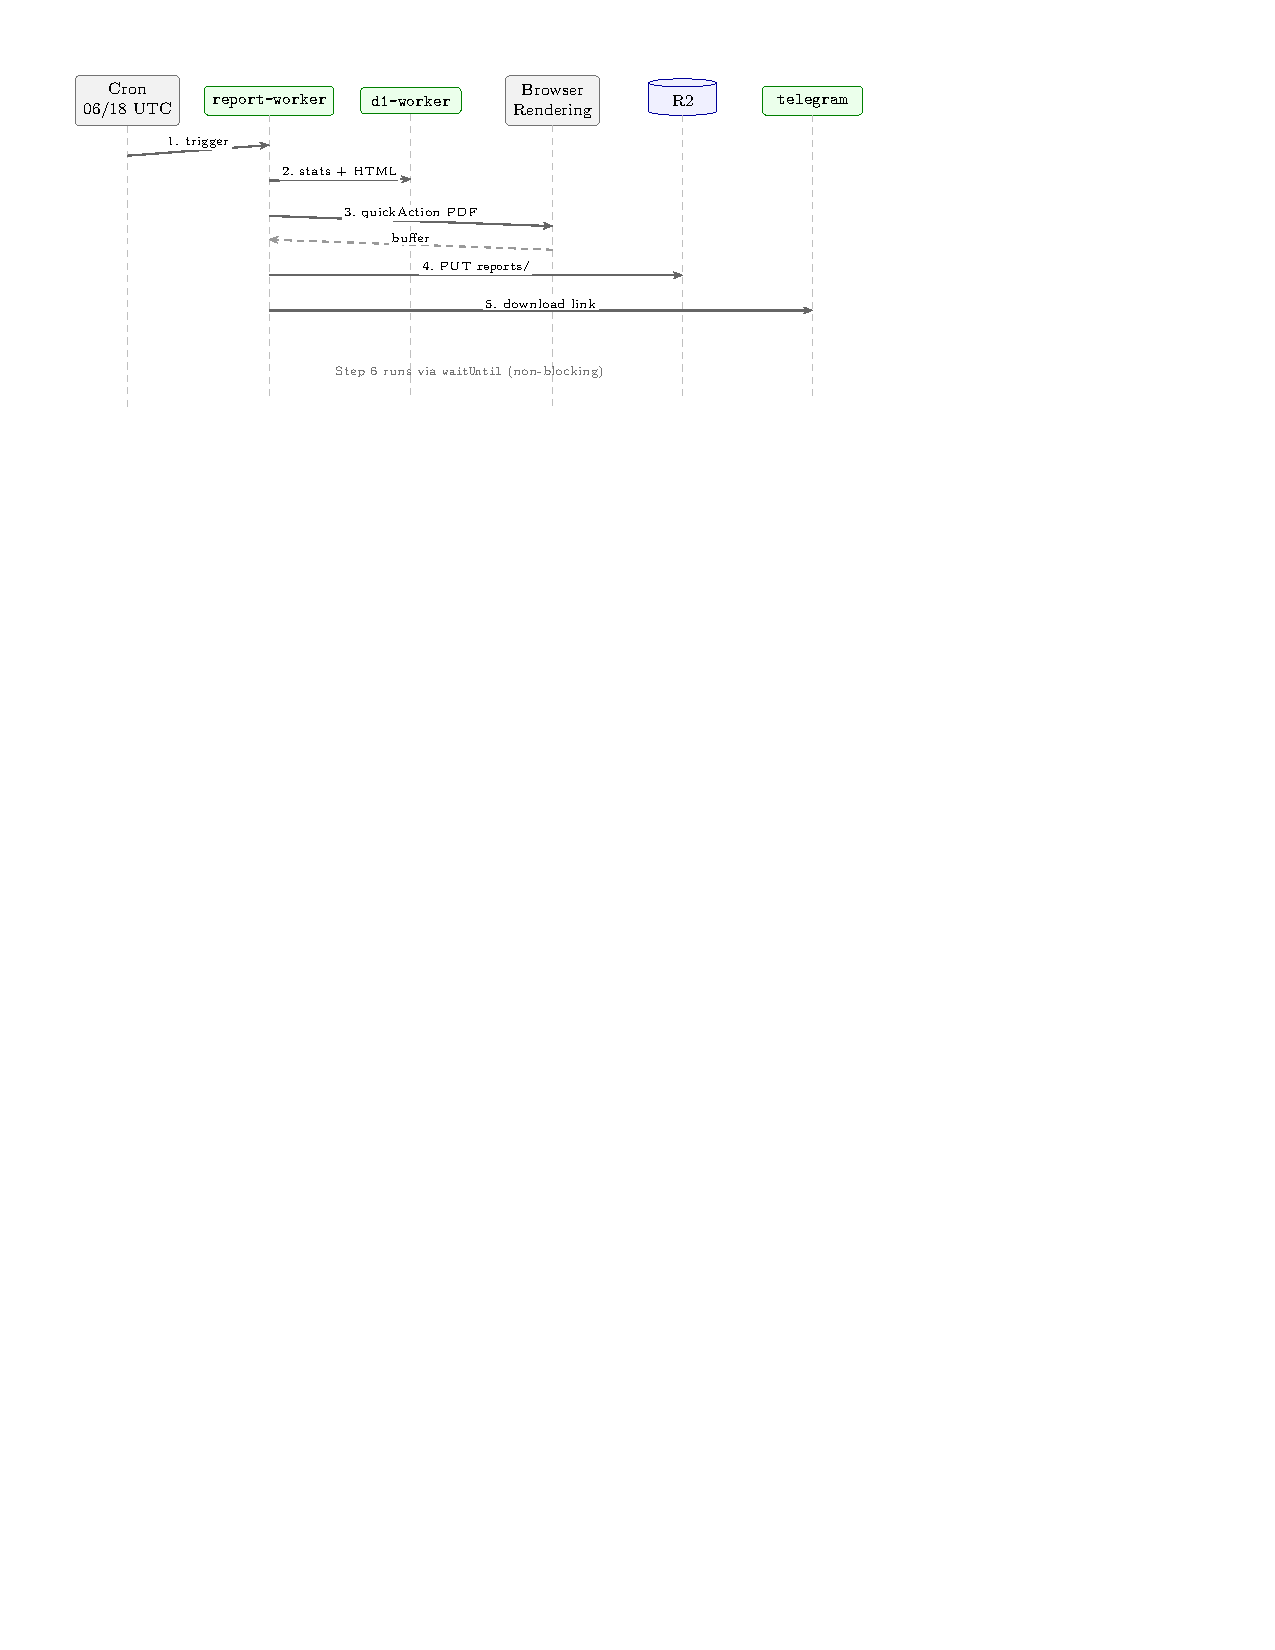
\includegraphics[width=0.98\linewidth]{figures/report-cron-lifecycle.pdf}%
  }{%
    \ifhooxusetikz
      \resizebox{0.98\linewidth}{!}{% TikZ sequence: report-worker scheduled PDF pipeline
\begin{tikzpicture}[
  actor/.style={draw=black!55, rounded corners=2pt, fill=gray!10,
    minimum width=1.7cm, minimum height=0.5cm, font=\footnotesize, align=center},
  worker/.style={draw=green!50!black, rounded corners=2pt, fill=green!8,
    minimum width=1.9cm, minimum height=0.5cm, font=\footnotesize\ttfamily, align=center},
  store/.style={draw=blue!60!black, cylinder, shape border rotate=90, aspect=0.22,
    fill=blue!6, minimum height=0.45cm, minimum width=1.3cm,
    font=\footnotesize, align=center},
  msg/.style={-{Stealth[length=1.5mm]}, semithick, draw=black!60},
  ret/.style={-{Stealth[length=1.5mm]}, semithick, dashed, draw=black!40},
  lifeline/.style={draw=black!25, dashed},
  msglabel/.style={font=\scriptsize, fill=white, inner sep=1pt}
]

  \node[actor] (cron) at (0,0) {Cron\\06/18 UTC};
  \node[worker] (rw) at (2.4,0) {report-worker};
  \node[worker] (d1) at (4.8,0) {d1-worker};
  \node[actor] (br) at (7.2,0) {Browser\\Rendering};
  \node[store] (r2) at (9.4,0) {R2};
  \node[worker] (tg) at (11.6,0) {telegram};

  \foreach \x in {cron,rw,d1,br,r2,tg} {
    \draw[lifeline] (\x.south) -- ++(0,-4.8);
  }

  \draw[msg] ([yshift=-0.5cm]cron.south) -- node[msglabel, above] {1.\ trigger} ([yshift=-0.5cm]rw.south);
  \draw[msg] ([yshift=-1.1cm]rw.south) -- node[msglabel, above] {2.\ stats + HTML} ([yshift=-1.1cm]d1.south);
  \draw[msg] ([yshift=-1.7cm]rw.south) -- node[msglabel, above] {3.\ quickAction PDF} ([yshift=-1.7cm]br.south);
  \draw[ret] ([yshift=-2.1cm]br.south) -- node[msglabel, above] {buffer} ([yshift=-2.1cm]rw.south);
  \draw[msg] ([yshift=-2.7cm]rw.south) -- node[msglabel, above] {4.\ PUT \texttt{reports/}} ([yshift=-2.7cm]r2.south);
  \draw[msg] ([yshift=-3.3cm]rw.south) -- node[msglabel, above] {5.\ download link} ([yshift=-3.3cm]tg.south);

  \node[font=\tiny, align=left, text=black!55] at (5.8,-4.6) {%
    Step 6 runs via \texttt{waitUntil} (non-blocking)%
  };

\end{tikzpicture}}%
    \else
      \fbox{\parbox{0.92\linewidth}{\small Cron $\rightarrow$ \texttt{report-worker} $\rightarrow$ \texttt{d1-worker} $\rightarrow$ Browser Rendering $\rightarrow$ R2 $\rightarrow$ Telegram}}
    \fi
  }
  \caption{\texttt{report-worker} scheduled PDF pipeline (06:00 and 18:00 UTC).}
  \label{fig:report-cron}
\end{figure}

\subsection{Dashboard (\texttt{dashboard})}

Next.js~16 application compiled with \texttt{@opennextjs/cloudflare}. Smart Placement is \emph{disabled}---the isolate runs near end-user browsers, not exchange APIs.

\paragraph{Architecture.} \texttt{.open-next/worker.js} handles SSR/RSC and API routes; \texttt{ASSETS} binding serves static chunks from the global CDN. API routes reach \texttt{d1-worker}, \texttt{analytics-worker}, and \texttt{agent-worker} via Service Bindings.

\paragraph{Bindings.} \texttt{D1\_SERVICE}, \texttt{ANALYTICS\_SERVICE}, \texttt{AGENT\_SERVICE}, \texttt{CONFIG\_KV}, \texttt{NEXT\_INC\_CACHE\_KV}.